\vzmstitle{ \bf  ИССЛЕДОВАНИЕ ТОПОЛОГИИ СЛОЕНИЯ ЛИУВИЛЛЯ ИНТЕГРИРУЕМОГО БИЛЛИАРДА В НЕВЫПУКЛЫХ ОБЛАСТЯХ}

\vzmsauthor{{Москвин}}{В.\, А.}

\vzmsinfo{Москва; {\it aoshi.k68@gmail.com}}

\addcontentsline{toc}{section}{Москвин В.А.\dotfill}

Биллиардная задача (биллиард) -- динамическая система, описывающая движение материальной точки внутри области с естественным абсолютно упругим отражением на границе (угол падения равен углу отражения). В книге С.Л. Табачникова [1] дан обзор современных исследований биллиардов. Для описания топологии совместных поверхностей уровня интегралов используется теория А.Т. Фоменко, которая в случае полных потоков изложена в книге Болсинова-Фоменко [2]. В настоящей работе ис\-следуют\-ся биллиарды, потоки в которых не являются полными. Это означает, что совместные поверхности уровня интегралов не являются торами. Рассмотрены биллиарды в невыпуклых областях, ограниченных дугами софокусных квадрик с ровно одной вершиной угла в $3\pi/2$ на границе области.
Траектории, попавшие в прямые углы, мы доопределим по непрерывности. Поступить так же с траекториями, попавшими в вершину тупого угла, сохраняя при этом непрерывность системы, невозможно.
Требование абсолютной упругости удара даёт нам первый интеграл -- квадрат длины вектора скорости, а теорема Якоби-Шаля гарантирует существования второго интеграла[1]. Исследование выполнено за счёт гранта Российского научного фонда (проект №17-11-01303).

\begin{figure}[h!]
	\center{ 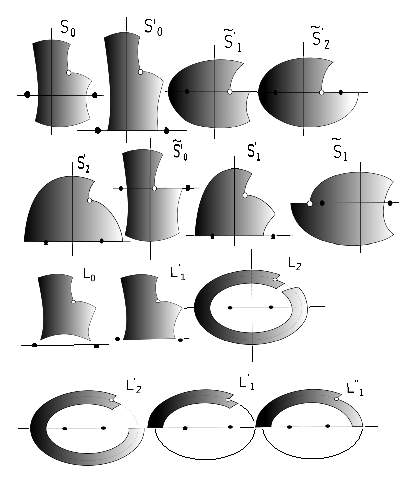
\includegraphics[width=100mm]{Moskvin_OblFull.eps}}
	\caption{Биллиардные области.}
\end{figure}

\textbf{Теорема~1.} {\it 	Любой элементарный биллиард такого вида эквивалентен одному из 14 биллиардов и принадлежит одной из следующих двух серий: \\
	1. Элементарные биллиарды серии $S$, содержащие отрезок фокальной прямой между фокусами. (внутри или на границе) Существует ровно 7 таких типов. Все такие биллиарды изображены на рисунке 1. \\
	2. Элементарные биллиарды серии $L$, которые не содержат отрезок фокальной прямой между фокусами. Такие билиарды имеют вид шестиугольника, ограниченного дугами эллипсов и гипербол, внутри или на границе области. Все такие биллиарды изображены на рисунке 1. Назовём их биллиардами типа $L$..} \\

\begin{figure}[h!]
	\center{ 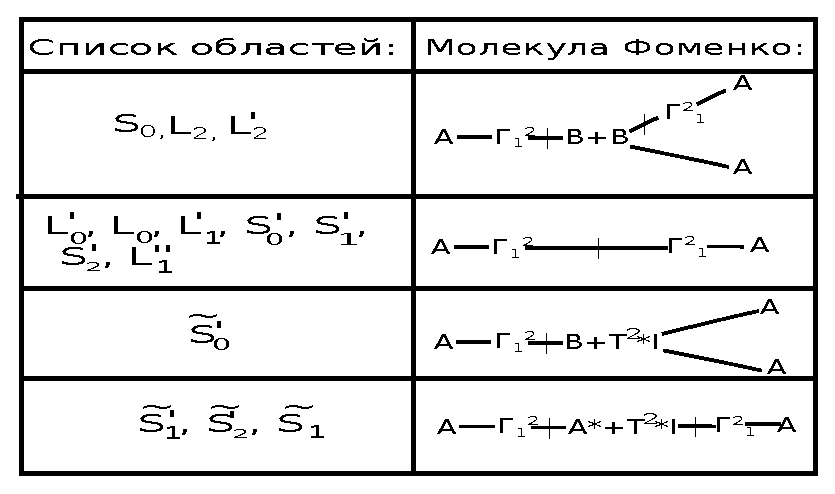
\includegraphics[width=70mm]{Moskvin_Table1.eps}}
	\caption{Молекулы Фоменко.}
\end{figure}

\textbf{Теорема~2.} {\it Для всех неособых значений интеграла повер\-хность уровня интеграла $\lambda$
	в изоэнергетичес\-кой поверхности $Q^3$ элементарного биллиарда $\Omega$ гомеоморфна объединению сфер с $k+1$ ручек и с $k$ выколотыми точками, где $k$ -- количество особых точек в проекции интегрального эллипса, если $\lambda<b$ или интегральной гиперболы, если $\lambda>b$.} \\
\textbf{Определение 1.} {\it
	Назовём $\Gamma^2_1$ прообаз значения интеграла $\varLambda = res \neq b$, если при увеличении параметра интегральной квадрики количество особых точек в интегральной области увеличится и $\Gamma^2_1$ в обратном случае. } \\
\textbf{Теорема~3.} {\it Для биллиардных областей, изображённых на рис.2, указанные молекулы Фоменко описывают топологию многообразия $Q^3$. }


\litlist

 1.  Геометрия и биллиарды. // С.\,Л.~Табачников. М.-Ижевск: НИЦ «Регулярная и хаотическая динамика», Ижевский институт компьютерных исследований,
2011 \\
2. Интегрируемые гамильтоновы системы. Геометрия, топология, классификация.// 	А.В. Болсинов, А.Т. Фоменко - том 1. Ижевск НИЦ	<<Регулярная и хаотическая динамика>>, 1999\\


